\documentclass[12pt]{article}
\usepackage[a4paper,left=3cm, right=1.5cm, top=2cm, bottom=2cm, headsep=1cm, footskip=1cm]{geometry}
\usepackage[utf8]{inputenc}
% \usepackage{natbib}
\usepackage{graphicx}
\usepackage{listings}
\usepackage{xcolor}
\usepackage[normalem]{ulem}
\definecolor{codegreen}{rgb}{0,0.6,0}
\definecolor{codegray}{rgb}{0.5,0.5,0.5}
\definecolor{codepurple}{rgb}{0.58,0,0.82}
\definecolor{backcolour}{rgb}{0.95,0.95,0.92}

\lstdefinestyle{mystyle}{
    basicstyle=\ttfamily\footnotesize,
    breakatwhitespace=false,
    breaklines=true,
    captionpos=b,
    keepspaces=true,
    numbers=left,
    numbersep=5pt,
    showspaces=false,
    showstringspaces=false,
    showtabs=false,
    tabsize=2
}

\lstset{style=mystyle}
\usepackage[english,russian]{babel}
\begin{document}
    \Large
    \begin{center}
        Санкт-Петербургский государственный университет\newline
        Прикладная математика и информатика\newline\newline\newline\newline\newline\newline
    \end{center}
    \begin{center}
        Отчёт по научно-исследовательской работе\newline
        Интегрирование дизайнов\newline\newline\newline\newline\newline
    \end{center}

    \hspace*{55mm}Выполнил:\newline
    \hspace*{61mm}Пономаренко А.В., группа 223\newline
    \hspace*{61mm}Научный руководитель:\newline
    \hspace*{61mm}Алексеева Н.П.\newline
    \hspace*{61mm}Кафедра статистического моделирования\newline\newline\newline\newline\newline\newline\newline
    \begin{center}
        Санкт-Петербург

        2019
    \end{center}
    \normalsize
    \newpage


    \section{Вступление}
    Часто в прикладных задачах встречается необходимость в планировании экспериментов. Для этого можно использовать теорию комбинаторных схем (дизайнов). Сейчас дизайны можно найти в широком ряде областей, включая конечную геометрию, математическую биологию, разработку и анализ алгоритмов, вычислительные сети, групповое тестирование и криптографию.\newline\newline
    Целью научно-исследовательской работы является изучение конечных геометрий и дизайнов с последующей реализацией алгоритма для интегрирования дизайнов.


    \section{Проективные геометрии}
    \textit{Проективные геометрии} — это раздел геометрии, изучающий проективные плоскости и пространства. Проективная геометрия может изучаться как с чисто геометрической точки зрения, так и с алгебраической, рассматривая проективную плоскость как структуру над полем.\newline

    \textbf{Проективное пространство можно определить с помощью разного набора аксиом:}
    \begin{enumerate}
        \itemСуществует прямая и точка не на ней.
        \itemНа каждой прямой есть по крайней мере три точки.
        \itemЧерез две точки можно провести ровно одну прямую.
        \itemЕсли A, B, C, и D — различные точки и AB и CD пересекаются, то AC и BD пересекаются.
        \itemЕсли ABC — плоскость, то существует по крайней мере одна точка не в плоскости ABC.
        \itemДве различные плоскости пересекаются по крайней мере в двух точках.
        \itemТри диагональные точки полного четырёхугольника не коллинеарны.
        \itemЕсли три точки на прямой X инвариантны по отношению к проективности $\phi$, то все точки на X инвариантны по отношению к $\phi$.\newline\newline
    \end{enumerate}

    \textbf{Проективная плоскость определяется несколько другими аксиомами:}
    \begin{enumerate}
        \item Через две точки можно провести ровно одну прямую.
        \item Любые две прямые пересекаются.
        \item Существует четыре точки, из которых нет трёх коллинеарных.
        \item Три диагональные точки полных четырёхугольников не коллинеарны.
        \item Если три точки на прямой X инвариантны по отношению к проективности $\phi$, то все точки на X инвариантны по отношению к $\phi$.
        \item Теорема Дезарга: Если два треугольника перспективны сквозь точку, то они перспективны сквозь прямую.\newline\newline
    \end{enumerate}

    Например, рассмотрим фигуру, состоящую из семи точек из семи прямых. Такая фигура называется фигурой Фано:
    \begin{figure}[h]
        \center{ 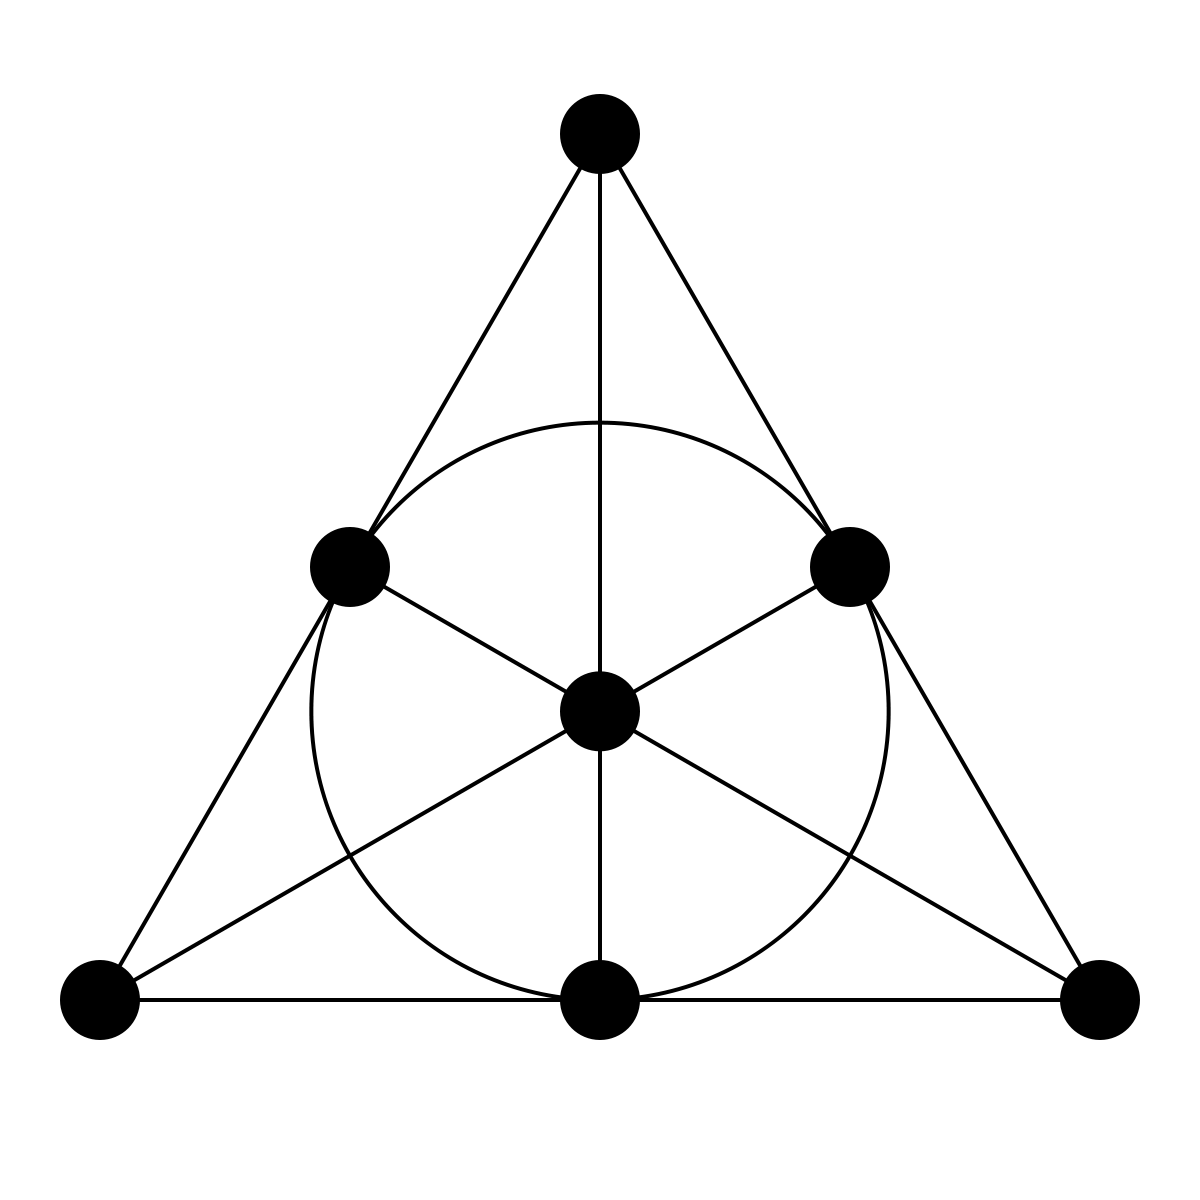
\includegraphics[scale = 0.15]{image.png}}
        \caption {Фигура Фано}
        \label{ris:image}
    \end{figure}
    \newline\newlineПусть $F_q$  произвольное поле характеристики $q$. Пространство векторов $(a_0, a_1, . . . , a_n)$, где $a_i \in F_q$, называется \textit{проективной геометрией размерности $n$ над $F_q$} и обозначается $PG(n, F_q)$ или $P^q_n$. Нулевой вектор - это пустое пространство размерности -1.\\ Точка P является пространством размерности 0 и представляет собой
    множество векторов $bx = b(x_0, . . . , x_n), x = (x_1, . . . , x_n) \neq 0, b \in F_q$.
    Если $y_0, . . . , y_k$  это независимые векторы, то множество векторов
    вида $b_0y_0 + ... + b_ky_k, где b_i \in F_q$, есть подпространство $S_k$. Подпространство $S_{n-1}$ называется \textit{гиперплоскостью}.


    \section{Конечные поля}
    Поле $F$ есть множество элементов с заданными операциями сложения и умножения, которые удовлетворяют аксиомам.\newline\newline
    \textbf{Аксиомы сложения:}
    \begin{enumerate}
        \item $\forall \, a, b \in F \,\,\, \exists \, c = a + b \in F$
        \item $(a + b) + c = a + (b + c)$
        \item $a + b = b + a;$
        \item $\exists \, 0 \in F, a + 0 = 0 + a = a$
        \item $\exists \, - a \in F, a + (-a) = 0;$\newline\newline\newline
    \end{enumerate}
    \textbf{Аксиомы умножения:}
    \begin{enumerate}
        \item $\forall \, a, b \in F \,\,\, \exists \, c = ab \in F$
        \item $(ab)c = a(bc)$
        \item $ab = ba$
        \item $\exists \, 1 \in F, a1 = 1a = a$
        \item $\exists \, a^{-1} \in F, aa^{-1} = 1$
    \end{enumerate}
    \textbf{Дистрибутивность:}
    \begin{enumerate}
        \item $a(b + c) = ab + ac$
    \end{enumerate}
    Приведем пример введения координат в конечной геометрии.
    Точками проективной геометрии $P^2_2$ являются векторы $(X_0, X_1, X_2)$
    с компонентами над $F_2$ кроме нулевого. Прямая, проходящая через
    точки $P_1$ и $P_2$, представляет собой совокупность точек вида: $u_1P_1+
    u_2P_2$ над $F_2$ , где $u_1, u_2 \in F_2, (u_1, u_2) \neq (0, 0)$. Таким образом, прямую образуют точки вида $(P_1, P_2, P_1 + P_2)$.


    \section{Дизайны}

    \subsection{Определение дизайна}
    Обозначим $v$ - множество элементов $m_{1}, m_{2}, ..., m_{v}$. Рассмотрим подмножества этого множества $M_{1}, M_{2}, ..., M_{b}$. Каждое подмножество $M_{j}$ называется \textit{блоком}, а число элементов множества $v$ в нем называется объемом блока и обозначается как $k$. Пусть $r$ - число подмножеств $M$, содержащих этот элемент. Число повторений (неупорядоченных пар) обозначается как $\lambda$. Тогда множество блоков $M_{1}, M_{2}, ..., M_{b}$ образует комбинаторную схему (или блок-схему) с параметрами $v, b, r, k, \lambda$.\newline
    Для $D(v, b, r, k, \lambda)$ справедливы два соотношения баланса:
    $$vr = bk, r(k - 1) = \lambda(v - 1)$$

    \subsection{Афинная геометрия}
    Пространство точек $(x_1, ... , x_n), x_i \in F_q$, называется аффинной
    геометрией и обозначается $E^q_n$.
    \textit{Остаточным} называется дизайн, который получается из блок-схемы при вычеркивании одного блока и всех его элементов из остальных блоков. Дизайн с блоками из вычеркнутых элементов называется \textit{производным}.\newline\newline
    Аксиомы афинной геометрии:
    \begin{enumerate}
        \item Для двух различных точек существует только одна прямая,
        которая содержит обе точки.
        \item  Для двух различных точек существует только одна прямая,
        которая содержит обе точки.
        \item Для прямой $P$ и точки $p \notin P$, существует одна и только одна
        прямая $P_0$, такая, что $p \in P_0, P \cap P_0 = \emptyset$.
    \end{enumerate}
    Для $P^q_n$ производный дизайн соответствует $P^q_{n-1}$, а остаточный $E^q_n$.
    Покажем это на примере дизайна $D(7, 3, 1)$. Удаляя из
    него элементы 1, 2, 3, получим остаточный дизайн $D(4, 6, 3, 2, 1)$,
    который состоит из $v = 4$ элементов $\{4, 5, 6, 7\}$ и $b = 6$ блоков.\newline\newline
    $$\begin{tabular}{  l l l  }
          (\sout{2}, 4, 6) \\
          (\sout{1}, 4, 5) \\
          (\sout{3}, 4, 7)\\
          (\sout{1, 2, 3}) & &  (4, 5) (6, 7)\\
          (\sout{2}, 5, 7) &  $\rightarrow$  & (4, 6) (5, 7)\\
          (\sout{1}, 6, 7) & &  (4, 7) (5, 6)\\
          (\sout{3}, 5, 6)\\

    \end{tabular}
    $$

    \subsection{Интегрирование дизайнов}
    \textit{Интегрированием дизайнов} называется процедура, противоположная разделению блок-схемы на производную и остаточную.
    В случае произвольной характеристики интегрирование дизайнов типа $P^q_n$ осуществляется на основе рекуррентных соотношений типа Фибоначчи, которые используются в алгебре в определении импульсных последовательностей.

    \subsubsection{Импульсные последовательности}
    Последовательность $\{\phi_j\}^\infty_{j=0}$ элементов конечного поля $F_q$, где $q = p^r$, называется \textit{импульсной}, если она получена в результате рекуррентного соотношения типа Фибоначчи:
    $$\phi_{j+1} = \phi_j + \alpha\phi_{j-1}, \alpha \in F_q$$

    \subsubsection{Пример интегрирования дизайнов}
    Рассмотрим проективную прямую $PG(1,4)$ с соответствующим вырожденным дизайном $D(5,1,0)$. Зададимся целью с помощью интегрирования дизайнов получить дизайн $D(21,5,1)$.
    Будем рассматривать в качестве элементов пять проективных векторов $(x_0, x_1)$ над $F_4$:

    $$
    \left( {\begin{array}{*{20}c}
                0  \\
                1  \\
    \end{array} } \right),
    \left( {\begin{array}{*{20}c}
                1  \\
                0  \\
    \end{array} } \right),
    \left( {\begin{array}{*{20}c}
                1  \\
                1  \\
    \end{array} } \right),
    \left( {\begin{array}{*{20}c}
                1  \\
                2  \\
    \end{array} } \right),
    \left( {\begin{array}{*{20}c}
                1  \\
                3  \\
    \end{array} } \right)
    $$

    Вложим наши вектора в пространство большей размерности, дополнив их дополнительной нулевой координатой. Таким образом, мы получим первый блок $B_1$:

    $$B_1 =
    \left( {\begin{array}{*{20}c}
                0 & 0 & 0 & 0 & 0  \\
                0 & 1 & 1 & 1 & 1\\
                1 & 0 & 1 & 2 & 3
    \end{array} } \right)
    $$
    Оставшиеcя блоки будем считать через импульсные последовательности. В роли $\phi_0$ будем брать пять элементов дизайна $D(5, 1, 0)$, а в качестве $\phi_1$ — вектора $(x_0, x_1)$ над $F_4$, вложенные в трехмерный вектор $(x_0, x_1, 1)$ с дополнительной единичной координатой. Например, по начальным условиям $\phi_0 = (1, 0, 0)$ и $\phi_1 = (0, 0, 1)$ строится проективный период импульсной последовательности с параметром рекуррентности $\alpha = 2$. Таким образом, блок $B_2$ имеет вид:
    $$B_2 =
    \left( {\begin{array}{*{20}c}
                0 & 1 & 1 & 1 & 1\\
                0 & 0 & 0 & 0 & 0\\
                1 & 0 & 2 & 3 & 1
    \end{array} } \right)
    $$

    Действуя аналогично, выбираем начальные условия с вектором $\phi_1$, который не лежит в предшествующих построенных блоках. То есть будем брать $\phi_1 \neq \phi_0$ для $B_3$ такой, что $\phi_1 \notin B_2$; для $B_4$ такой, что $\phi_1 \notin \{B_2,B_3\}$; для $B_5$ такой, что $\phi_1 \notin \{B_2,B_3,B_4\}$. Таким образом мы получим соответствующие блоки для фиксированного $\phi_0$:
    $$B_3 =
    \left( {\begin{array}{*{20}c}
                0 & 1 & 1 & 1 & 1\\
                0 & 1 & 1 & 1 & 1\\
                1 & 0 & 2 & 3 & 1
    \end{array} } \right),
    B_4 =
    \left( {\begin{array}{*{20}c}
                0 & 1 & 1 & 1 & 1\\
                0 & 2 & 2 & 2 & 2\\
                1 & 0 & 2 & 3 & 1
    \end{array} } \right),
    B_5 =
    \left( {\begin{array}{*{20}c}
                0 & 1 & 1 & 1 & 1\\
                0 & 3 & 3 & 3 & 3\\
                1 & 0 & 2 & 3 & 1
    \end{array} } \right)
    $$

    Поступая по аналогии, для остальных блоков исходного дизайна $D(5, 1, 0)$ построим остальные 16 блоков нового дизайна $D(21,5,1)$:\\\\\\
    $B_6 =
    \left( {\begin{array}{*{20}c}
                0 & 1 & 1 & 1 & 1\\
                1 & 0 & 2 & 3 & 1\\
                0 & 0 & 0 & 0 & 0
    \end{array} } \right),
    B_7 =
    \left( {\begin{array}{*{20}c}
                0 & 1 & 1 & 1 & 1\\
                1 & 0 & 2 & 3 & 1\\
                0 & 1 & 1 & 1 & 1
    \end{array} } \right),
    B_8 =
    \left( {\begin{array}{*{20}c}
                0 & 1 & 1 & 1 & 1\\
                1 & 0 & 2 & 3 & 1\\
                0 & 2 & 2 & 2 & 2
    \end{array} } \right),\\\\\\\\
    B_9 =
    \left( {\begin{array}{*{20}c}
                0 & 1 & 1 & 1 & 1\\
                1 & 0 & 2 & 3 & 1\\
                0 & 3 & 3 & 3 & 3
    \end{array} } \right),
    B_{10} =
    \left( {\begin{array}{*{20}c}
                0 & 1 & 1 & 1 & 1\\
                1 & 0 & 2 & 3 & 1\\
                1 & 0 & 2 & 3 & 1
    \end{array} } \right),
    B_{11} =
    \left( {\begin{array}{*{20}c}
                0 & 1 & 1 & 1 & 1\\
                1 & 1 & 3 & 2 & 0\\
                1 & 0 & 2 & 3 & 1
    \end{array} } \right),\\\\\\\\
    B_{12} =
    \left( {\begin{array}{*{20}c}
                0 & 1 & 1 & 1 & 1\\
                1 & 2 & 0 & 1 & 3\\
                1 & 0 & 2 & 3 & 1
    \end{array} } \right),
    B_{13} =
    \left( {\begin{array}{*{20}c}
                0 & 1 & 1 & 1 & 1\\
                1 & 3 & 1 & 0 & 2\\
                1 & 0 & 2 & 3 & 1
    \end{array} } \right),
    B_{14} =
    \left( {\begin{array}{*{20}c}
                0 & 1 & 1 & 1 & 1\\
                1 & 0 & 2 & 3 & 1\\
                2 & 0 & 3 & 1 & 2
    \end{array} } \right),\\\\\\\\
    B_{15} =
    \left( {\begin{array}{*{20}c}
                0 & 1 & 1 & 1 & 1\\
                1 & 1 & 3 & 2 & 0\\
                2 & 0 & 3 & 1 & 2
    \end{array} } \right),
    B_{16} =
    \left( {\begin{array}{*{20}c}
                0 & 1 & 1 & 1 & 1\\
                1 & 2 & 0 & 1 & 3\\
                2 & 0 & 3 & 1 & 2
    \end{array} } \right),
    B_{17} =
    \left( {\begin{array}{*{20}c}
                0 & 1 & 1 & 1 & 1\\
                1 & 3 & 1 & 0 & 2\\
                2 & 0 & 3 & 1 & 2
    \end{array} } \right),\\\\\\\\
    B_{18} =
    \left( {\begin{array}{*{20}c}
                0 & 1 & 1 & 1 & 1\\
                1 & 0 & 2 & 3 & 1\\
                3 & 0 & 1 & 2 & 3
    \end{array} } \right),
    B_{19} =
    \left( {\begin{array}{*{20}c}
                0 & 1 & 1 & 1 & 1\\
                1 & 1 & 3 & 2 & 0\\
                3 & 0 & 1 & 2 & 3
    \end{array} } \right),
    B_{20} =
    \left( {\begin{array}{*{20}c}
                0 & 1 & 1 & 1 & 1\\
                1 & 2 & 0 & 1 & 3\\
                3 & 0 & 1 & 2 & 3
    \end{array} } \right),\\\\\\\\
    B_{21} =
    \left( {\begin{array}{*{20}c}
                0 & 1 & 1 & 1 & 1\\
                1 & 3 & 1 & 0 & 2\\
                3 & 0 & 1 & 2 & 3
    \end{array} } \right)$\\\\\\\\\\\\\\\\\\\\

    Остаётся проверить, что построенные нами блоки это действительно элементы нужного дизайна.
    Будем считать, что входные данные — это полученные в результате работы рекуррентного алгоритма блоки,
    элементы которых записаны через запятую в формате csv.
    Для проверки условий воспользуемся небольшой программой на языке Python:
    \begin{lstlisting}[language=Python]
import numpy as np
import pandas as pd

data = pd.read_csv("blocks", header=None)

    aa = []
    k = 0
    l = 0
    for i, j in data.iterrows():
    if k == 0:
    block = j
    if k != 0:
    block = np.vstack((block, j))
    k += 1

    if k == 3:
    aa.append(block)

    k = 0
    if l == 0:
    bb = block
    else:
    bb = np.hstack((bb, block))
    l += 1
    block = []
    ll = []
    for i in bb.T:
    ll.append(tuple(i))

    my_set = set()
    for l in ll:
    my_set.add(l)

    for i in my_set:
    print('Vector', i, 'repeats', ll.count(i), 'times')

    pairs = set()
    temp = []
    for i in aa:
    i = i.T
    for j in range(len(i) - 1):
    t1 = tuple(np.hstack((i[j], i[j + 1])))
    t2 = tuple(np.hstack((i[j + 1], i[j])))
    temp.append(t1)
    temp.append(t2)
    pairs.add(t1)
    pairs.add(t2)

    for i in pairs:
    print('Pair', i, 'repeats', temp.count(i), 'times')
    \end{lstlisting}\leavevmode \\\\\\\\\\\\

    В результате работы алгоритма на представленных выше блоках, получим вывод:
    \small
    \begin{lstlisting}
Vector (0, 1, 1) repeats 5 times
    Vector (1, 0, 3) repeats 5 times
    Vector (1, 3, 2) repeats 5 times
    Vector (0, 1, 2) repeats 5 times
    Vector (1, 0, 0) repeats 5 times
    Vector (1, 3, 1) repeats 5 times
    Vector (0, 1, 3) repeats 5 times
    Vector (1, 0, 1) repeats 5 times
    Vector (1, 3, 0) repeats 5 times
    Vector (1, 0, 2) repeats 5 times
    Vector (1, 2, 0) repeats 5 times
    Vector (1, 2, 1) repeats 5 times
    Vector (1, 2, 2) repeats 5 times
    Vector (0, 0, 1) repeats 5 times
    Vector (1, 2, 3) repeats 5 times
    Vector (1, 1, 1) repeats 5 times
    Vector (1, 1, 0) repeats 5 times
    Vector (1, 1, 3) repeats 5 times
    Vector (1, 1, 2) repeats 5 times
    Vector (0, 1, 0) repeats 5 times
    Vector (1, 3, 3) repeats 5 times
    \end{lstlisting}
    \begin{lstlisting}
Pair (1, 1, 0, 1, 3, 3) repeats 1 times
    Pair (1, 2, 2, 1, 0, 1) repeats 1 times
    Pair (1, 0, 2, 1, 2, 1) repeats 1 times
    \end{lstlisting}
    ...
    \begin{lstlisting}[firstnumber=166]
Pair (1, 1, 2, 1, 3, 3) repeats 1 times
    Pair (1, 2, 2, 1, 3, 3) repeats 1 times
    Pair (1, 0, 2, 1, 1, 3) repeats 1 times
    \end{lstlisting} \leavevmode
    \normalsize
    Таким образом, мы получили $v=21$ элемент и $b=21$ блок размера $k=5$, каждый элемент которого встречается ровно $r=5$ раз. А каждая пара встречаются ровно $\lambda=1$ раз. Это и означает, что мы получили нужный дизайн $D(v,b,r,k,\lambda) = D(21,5,1)$


    \section{Заключение}
    В результате выполнения научно-исследовательской работы был изучен раздел комбинаторики, связанный с комбинаторными схемами (дизайнами) и их интегрированием, раздел алгебры, связанный с конечными полями и соответствующий раздел геометрии, связанный с конечными геометриями.


    \section{Список литературы}
    \begin{itemize}
        \item Алексеева Н.П. Анализ медико-биологических систем. Реципрокность, эргодичность, синонимия. — Издательство С.-Петербургского университета, 2012.
        \item Холл М. Комбинаторика. — МИР, 1970. 424c.
        \item Stinson Douglas R. Combinatorial Designs: Constructions and Analysis. — New York: Springer, 2003.
    \end{itemize}

\end{document}